
\section{Second-Order Model}
We will use \gls{second-order model} as shorthand for a linear, ordinary, time-invariant second-order differential equation of the form
\begin{equation} \label{e:second}
\ddot{y}(t) + 2 \zeta \omega_n \dot{y}(t) + \omega_n^2 y(t) = f(t)
\end{equation} 
where 
\begin{itemize}
\item $\ddot{y}(t)$ is the second derivative of $y(t)$ with respect to time,
\item $\dot{y}(t)$ is the first derivative of $y(t)$ with respect to time,
\item $y(t)$ is the solution to (\ref{e:second}),
\item $\zeta$ is the \gls{damping ratio},
\item $\omega_n$ is the \gls{undamped natural frequency} and
\item $f(t)$ is the input, or forcing function.
\end{itemize}
Just as with our first-order and static (zero-order) models, this model is an abstraction; it never has exactly the same behavior of a physical system, but it has been proven to be a useful approximation for the behavior of a variety of phenomena.  To understand the model we'll first present the solution to (\ref{e:second}) for a few types of input (forcing functions) and then work through some examples of cases where the model is a helpful abstraction of physical systems.

The intent of the following discussion is meant to be a summary and/or review of what you have seen in other courses (Differential Equations, System Dynamics, Feedback Controls, etc.).  The discussion should be sufficient for our purposes of modeling and measurement, but it is by no means an exhaustive treatment of analysis of second-order models or harmonic oscillator models.

Also, for now we are only interested in {\bf underdamped} and {\bf undamped} versions of the model (\ref{e:second}) where $0 \leq \zeta < 1.0$.  Another way to say this is that we are only interested in second-order models that have oscillations in their response.

\subsection{Example: Mass-Spring-Damper}
One type of physical system that has similar behavior to our second-order model is the mass-spring-damper system illustrated in Figure~\ref{f:msd2}.  (Actually, this system is still a bit of an abstraction; we rarely encounter applications that require a point mass attached to a mass-less spring.  The abstraction is meant to represent any physical system where there is inertia (mass, kinetic energy), a restoring force (spring, potential energy) and motion resistance (damper, energy dissipation).)
\begin{figure}[htb!]
\centerline{
{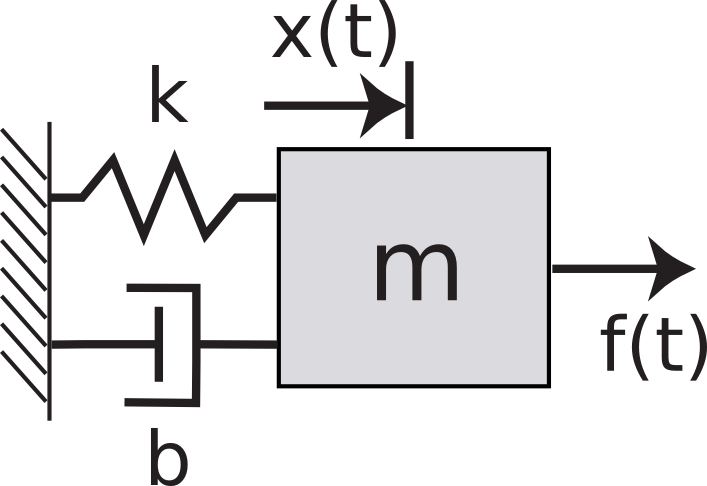
\includegraphics[width=0.4\textwidth]{msd_lower.png}}}
\caption{Sketch of a mass-spring-damper system.}
\label{f:msd2}
\end{figure}

If you draw a free-body-diagram of this system, you should be able to derive the second-order equation of motion
\begin{equation}\label{e:msd}
m \ddot{x}(t) + b \dot{x}(t) + k x(t) = f(t)
\end{equation}
where $m$ is the mass, $b$ is the linear damping coefficient, $k$ is the linear spring constant, $x(t)$ is the displacement of the mass and $f(t)$ is the input force.

\begin{ex}
Using (\ref{e:second}) and (\ref{e:msd}), derive expressions for the system parameters ($\omega_n$ and $\zeta$) in terms of the physical parameters ($m$, $b$, and $k$).  (Hint: Use physical units to check your answers.)
\end{ex}

\ifsolutions
\begin{soln}
You should verify that the following expressions are correct:
\[ \omega_n = \sqrt{k/m} \; \; \; \unitfrac[]{rad}{s}\]
\[ \zeta = \frac{b}{2 \sqrt{mk}} \; \; \; \unitfrac[]{n}{a} \]
\end{soln}
\fi


\section{Free Response}\label{s:secondfree}
The free response for our model is the solution to the second-order model (\ref{e:second}) with initial conditions, but no forcing function (also known as the homogeneous equation)
\begin{equation} \label{e:secondhomo}
\ddot{y}(t) + 2 \zeta \omega_n \dot{y}(t) + \omega_n^2 y(t) = 0
\end{equation} 
where the initial conditions at $t=0$ are
\begin{itemize}
\item $y(0) = y_o$ and 
\item $\dot{y}(0)=\dot{y}_o$.
\end{itemize}
Hopefully you've been convinced that this type of differential equation is straightforward to solve (in theory), and we can present (without derivation) that the solution to this equation is the function
\begin{equation} \label{e:secondfree}
y(t) = C \left(e^{-\zeta \omega_n t}\right) \left( \cos(\omega_d t - \phi) \right).
\end{equation}
where
\begin{eqnarray}\
\omega_d & = & \omega_n \sqrt{1-\zeta^2}, \label{e:damped} \\
C & = & \sqrt{ y_o^2 + \left( \frac{\dot{y}_o+\zeta\omega_n y_o}{\omega_d} \right)^2 } \;\;\;\;\;\;\;\;\; \mathrm{and}\label{e:C} \\
\tan(\phi) & = & \frac{\dot{y}_o+\zeta \omega_n y_o}{\omega_d y_o}. \label{e:phi}
\end{eqnarray}

The free response (\ref{e:secondfree}) is the key part of all this.  There are many systems that behave in this general way with a decaying oscillatory response.  To illustrate this we can annotate the equation to highlight the three parts of the solution:
\begin{equation} \label{e:secondfree_annote}
y(t) = \underbrace{C}_\text{constant} 
\underbrace{\left(e^{-\zeta \omega_n t}\right)}_\text{exponential decay}
\underbrace{\left( \cos(\omega_d t - \phi) \right)}_\text{oscillation}.
\end{equation}
One important detail is that there are two slightly different ``natural frequencies'' to keep track of.  The \gls{undamped natural frequency} ($\omega_n$) is the parameter we saw in the system model and which is included in the exponential decay component of (\ref{e:secondfree_annote}).  The \gls{damped natural frequency} ($\omega_d$) is the frequency of oscillation, the angular frequency inside the $\cos$ term of (\ref{e:secondfree_annote}).  The relation between the two values is given in (\ref{e:damped}).  For small values of $\zeta$, so called ``lightly damped systems'', there is little difference between the two values.

Another way to ``see'' this solution is to graph the time response.  The short MATLAB script in Listing~\ref{l:secondfree} generates Figure~\ref{f:secondfree}.  This figure illustrates the key characteristics of a second order free response:
\begin{enumerate}
\item the system oscillates at a constant frequency (the $\cos(\omega_d t)$ term) and
\item the amplitude of the oscillations decays exponentially over time (the $e^{=\zeta \omega_n t}$ term).
\end{enumerate}
%\lstinputlisting[style=myMatStyle,
%caption={Script for plotting the free response of a second-order model (\verb+second_order_free.m+).},
%label={l:second_free}]
%{./code/second_order_free.m}

\lstinputlisting[style=myMatStyle,
caption={Script for plotting the free response of a second-order model. (Filename=second\_order\_free.m, \url{http://web.eng.hawaii.edu/~bsb/me402/book/code/second_order_free.m})},
label={l:secondfree}]
{../code/second_order_free.m}


\begin{figure}[hbt]
\centering
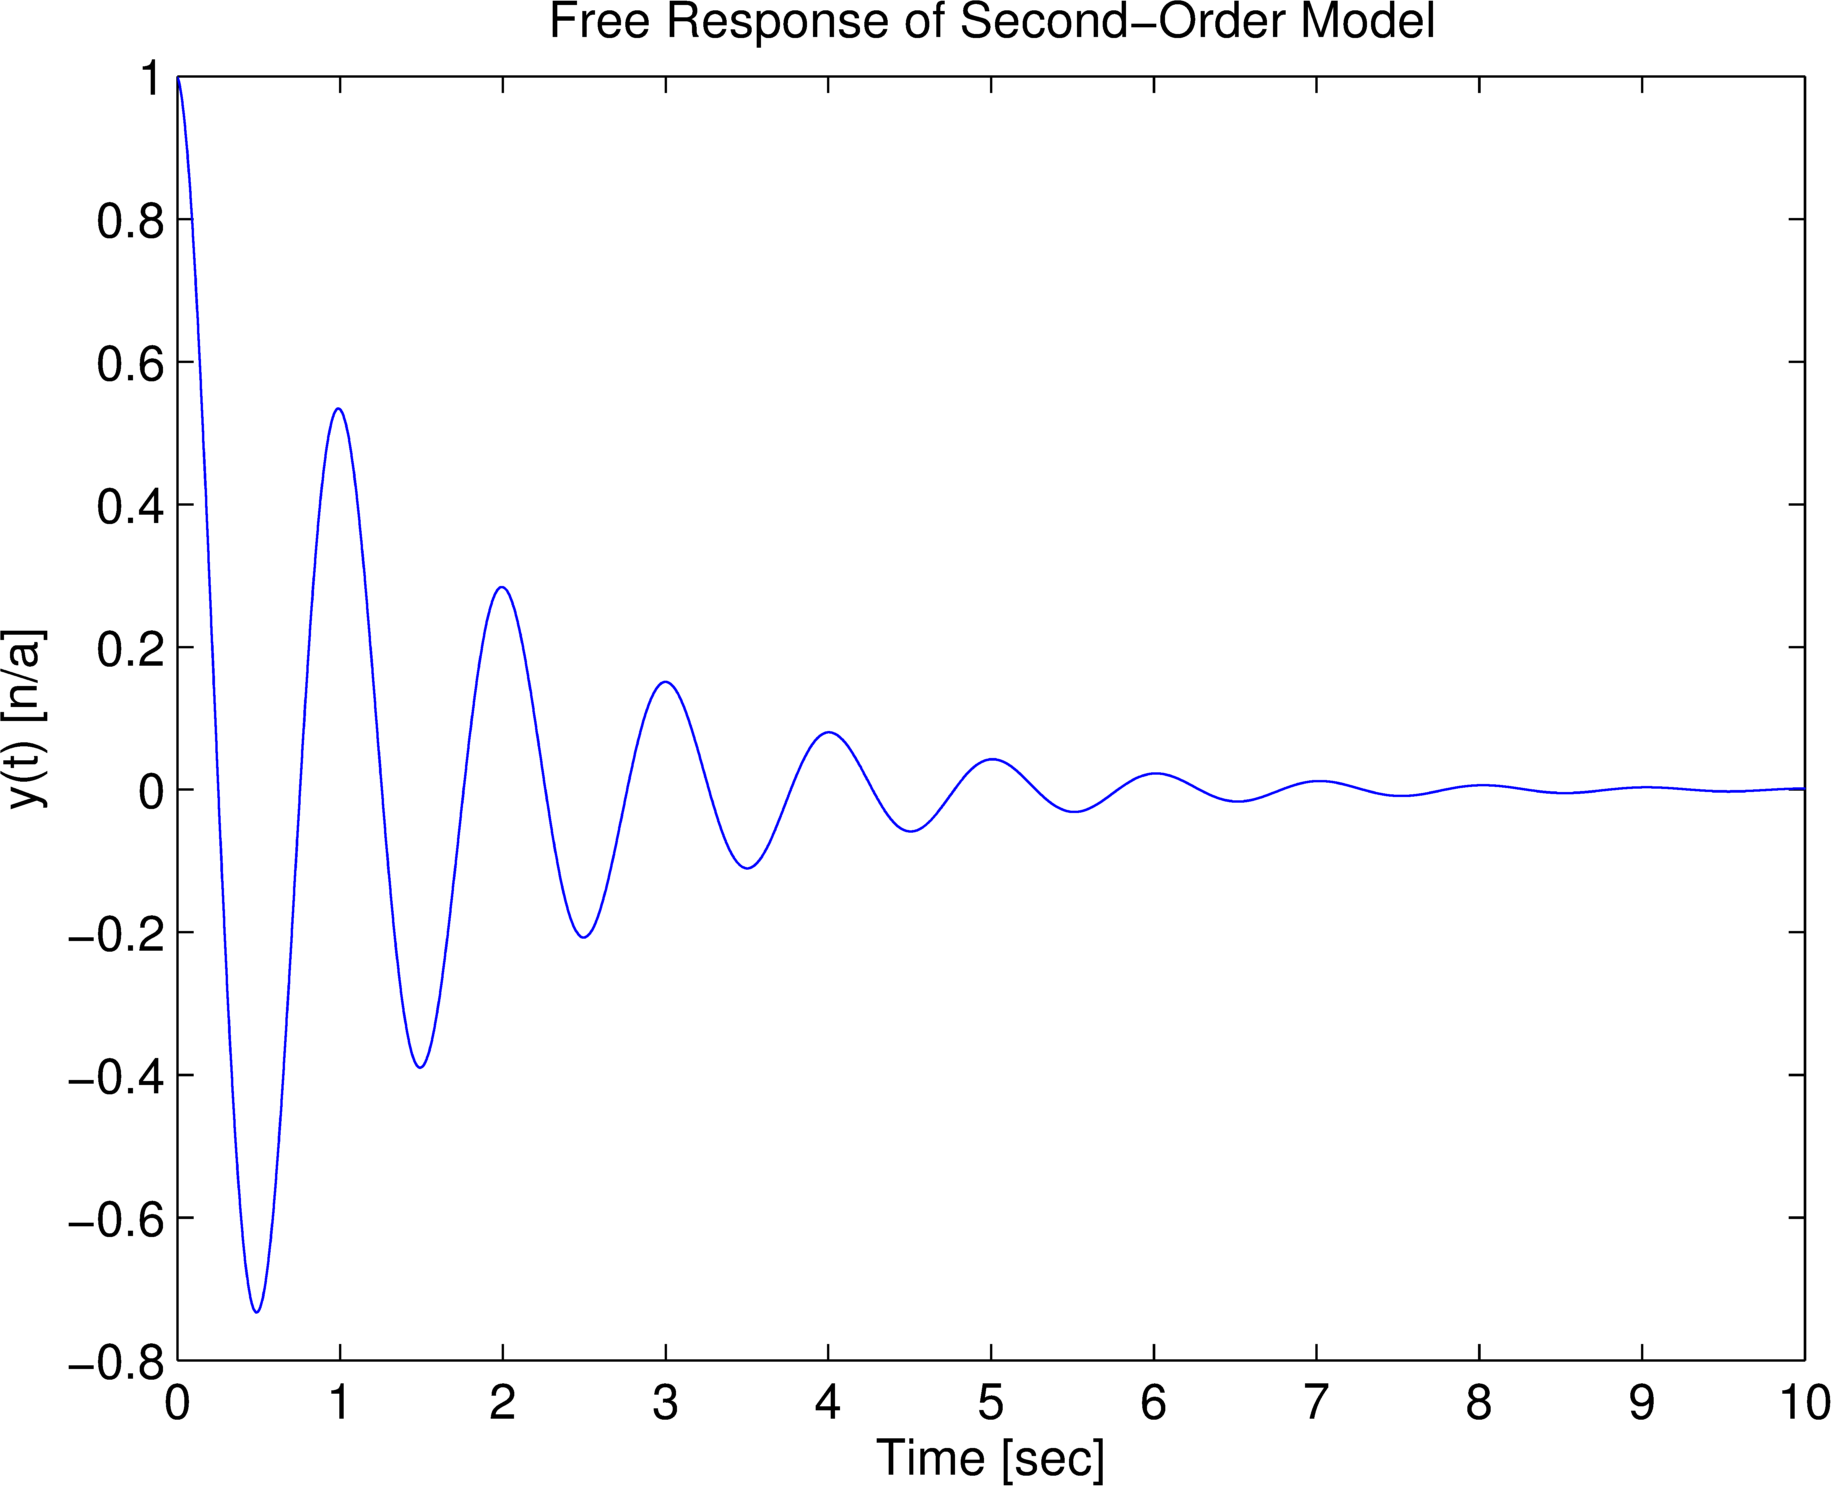
\includegraphics[width=\FigWidth\textwidth]{second_free.png}
\caption{Graph of the free response (\ref{e:stepresp}) with $\omega_n= \unit[1]{Hz}$, $\zeta=0.1$ (10\%) and $y(t=0)=1$.}
\label{f:secondfree}
\end{figure}

\begin{ex}
There is a mistake in Listing~\ref{l:secondfree} which attempted to display the solution for the case where there is only a ``displacement'' initial condition: i.e., $y(0)=y_o$ and $\dot{y}(0)=0$.  The mistake is that the solution in the code uses the values $C=y_o$ and $\phi=0$ which are not correct (but they are close). 
\begin{itemize}\label{ex:secondresp}
\item Derive expressions for the constants $C$ and $\phi$ based on the initial conditions $y(0)=y_o$ and $\dot{y}(0)=0$.
\item Copy the script in Listing~\ref{l:secondfree} and create the graph shown in Figure~\ref{f:secondfree}.
\item Correct the script in Listing~\ref{l:secondfree} and plot a second curve, on the same axes, with the corrected solution for $y_o=1$.  
  \begin{itemize}
  \item Include your MATLAB script with your solution.
  \item Include your graph as a properly formatted figure.
  \end{itemize}
\end{itemize}
The error is simply in the calculation of $C$ and $\phi$; the structure of the script in Listing~\ref{l:secondfree} should work just fine.
\end{ex}

\ifsolutions
\begin{soln}
\[ C = \sqrt{\frac{y_o}{1-\zeta^2}} \]
\[ \tan\phi = \frac{\zeta}{\sqrt{1-\zeta^2}} \]
or 
\[ \phi = \arctan\left(\frac{\zeta}{\sqrt{1-\zeta^2}}\right) \]

See Figure~\ref{f:secondfreesoln}.  This figure is generated using Listing~\ref{l:seconfree2}

\lstinputlisting[style=myMatStyle,
caption={Script for plotting the corrected free response of a second-order model.},
label={l:secondfree2}]
{../code/second_order_free_correct.m}

\begin{figure}[hbt]
\centering
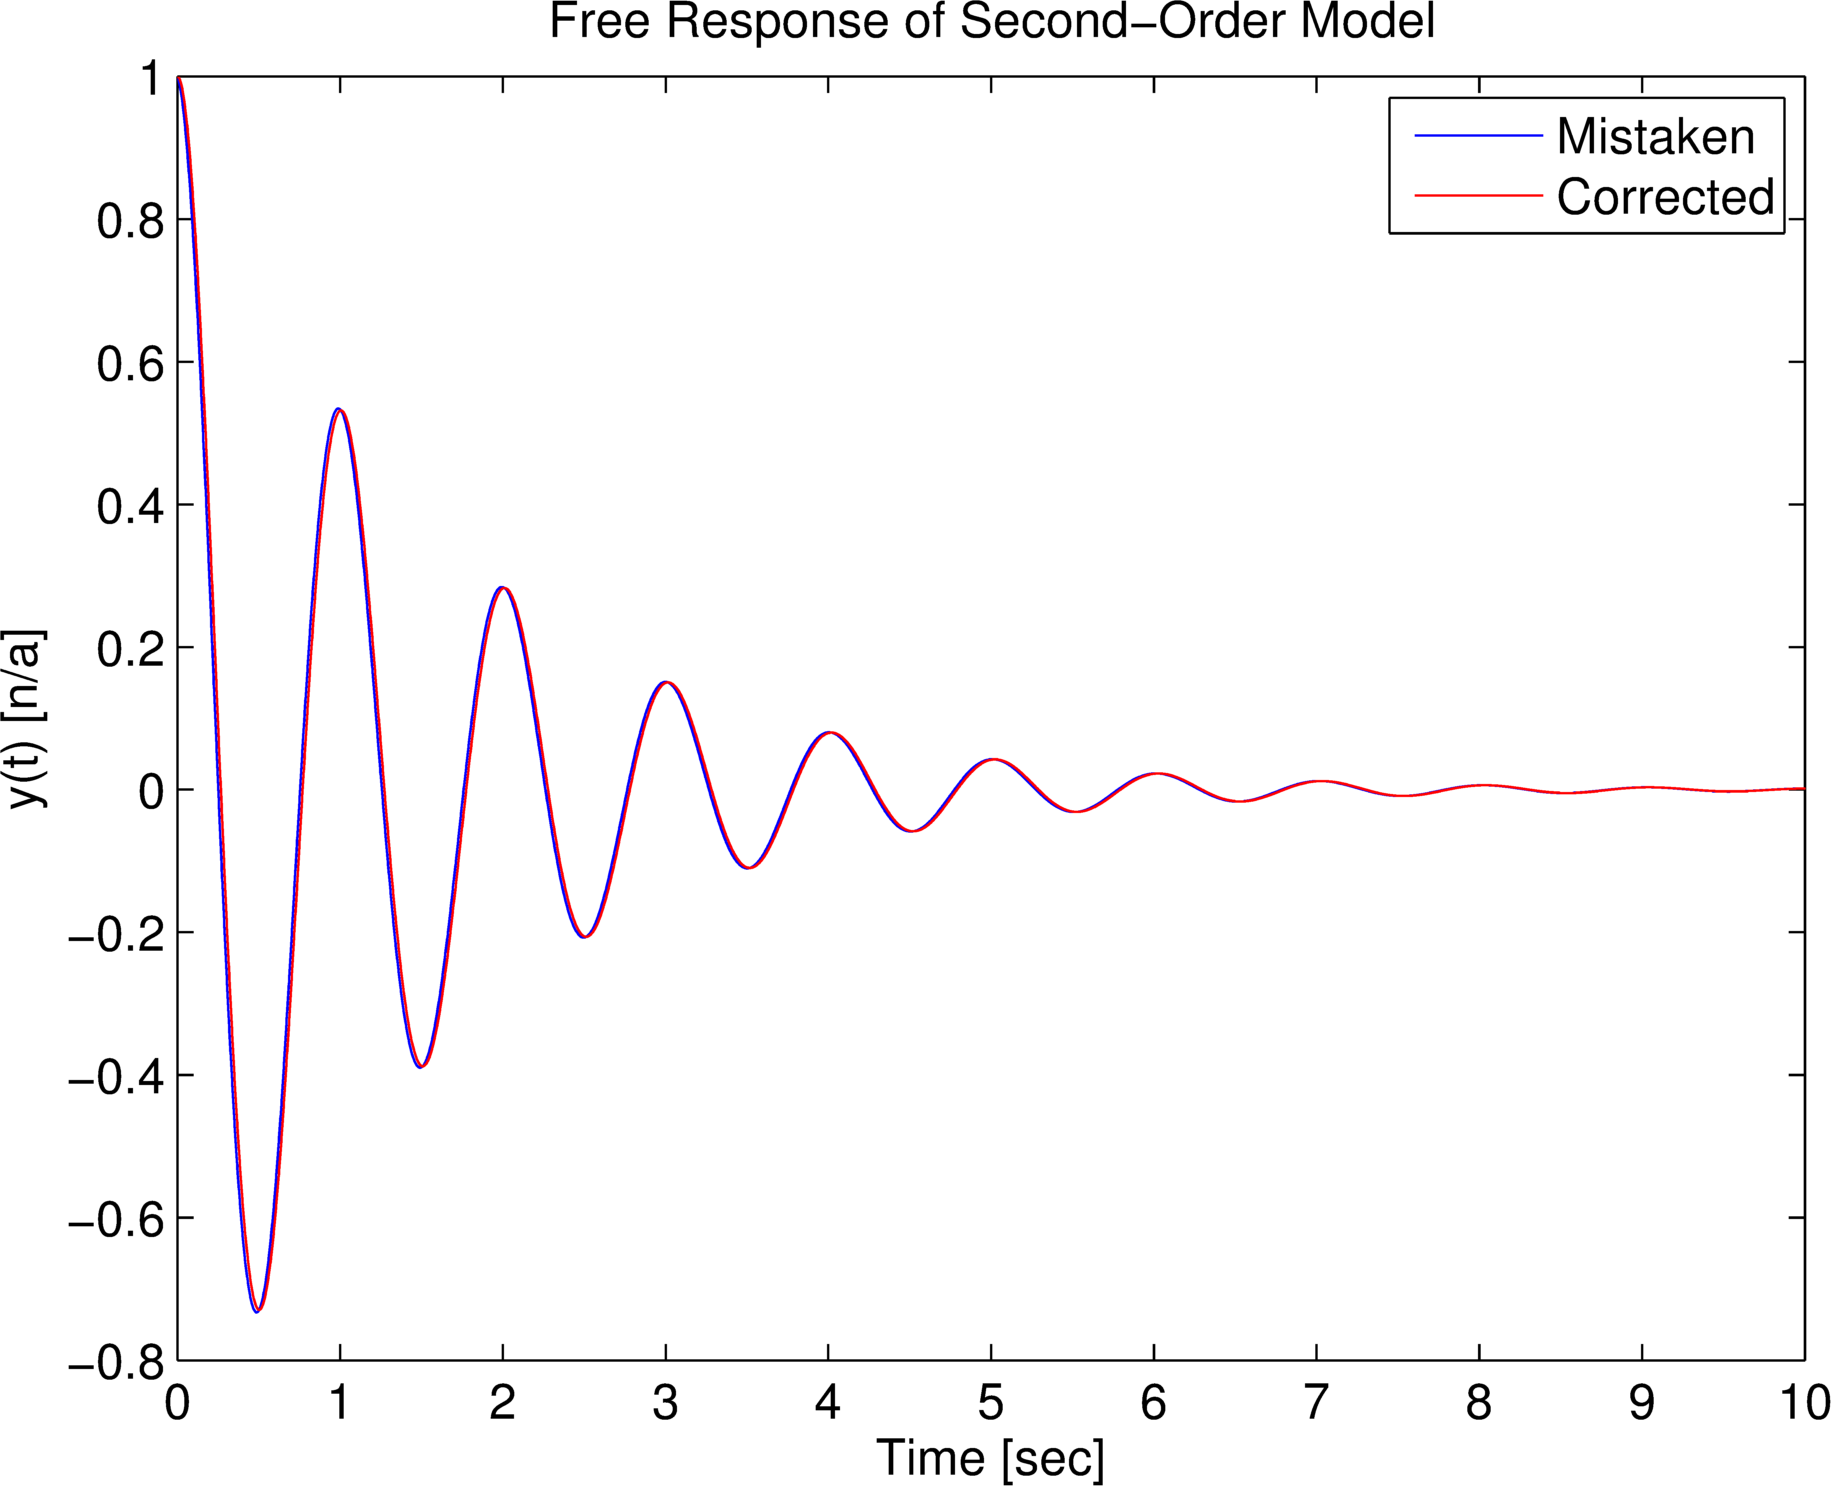
\includegraphics[width=\FigWidth\textwidth]{second_free_soln.png}
\caption{Graphs of the original mistaken free response and the corrected free response.}
\label{f:secondfreesoln}
\end{figure}
\end{soln}
\fi

\begin{ex}
Consider the effect of the damping ratio ($\zeta$) on the shape of free response.  Using Listing~\ref{l:secondfree} as a starting point, use MATLAB to create a single graph for the free response with the initial conditions $y(0)=1$ and $\dot{y}(0)=0$.  On a single set of axes, plot the response for systems with the following values for the damping ratio: $\zeta=\{0.0, 0.01 , 0.1, 0.5, 0.9\}$.  Use a legend to declare which curve is associated with each value of $\zeta$.  Submit this single graph as an appropriately formatted figure with a short description of what you observe about the effect of changing $\zeta$.
\end{ex}

\ifsolutions
\begin{soln}
See Figure~\ref{f:secondfreezetas} generated using Listing~\ref{l:secondfreezeta}.

\lstinputlisting[style=myMatStyle,
caption={Script for plotting the free response of a second-order model with varios values of zeta.},
label={l:secondfreezeta}]
{../code/second_order_free_zeta.m}


\begin{figure}[hbt]
\centering
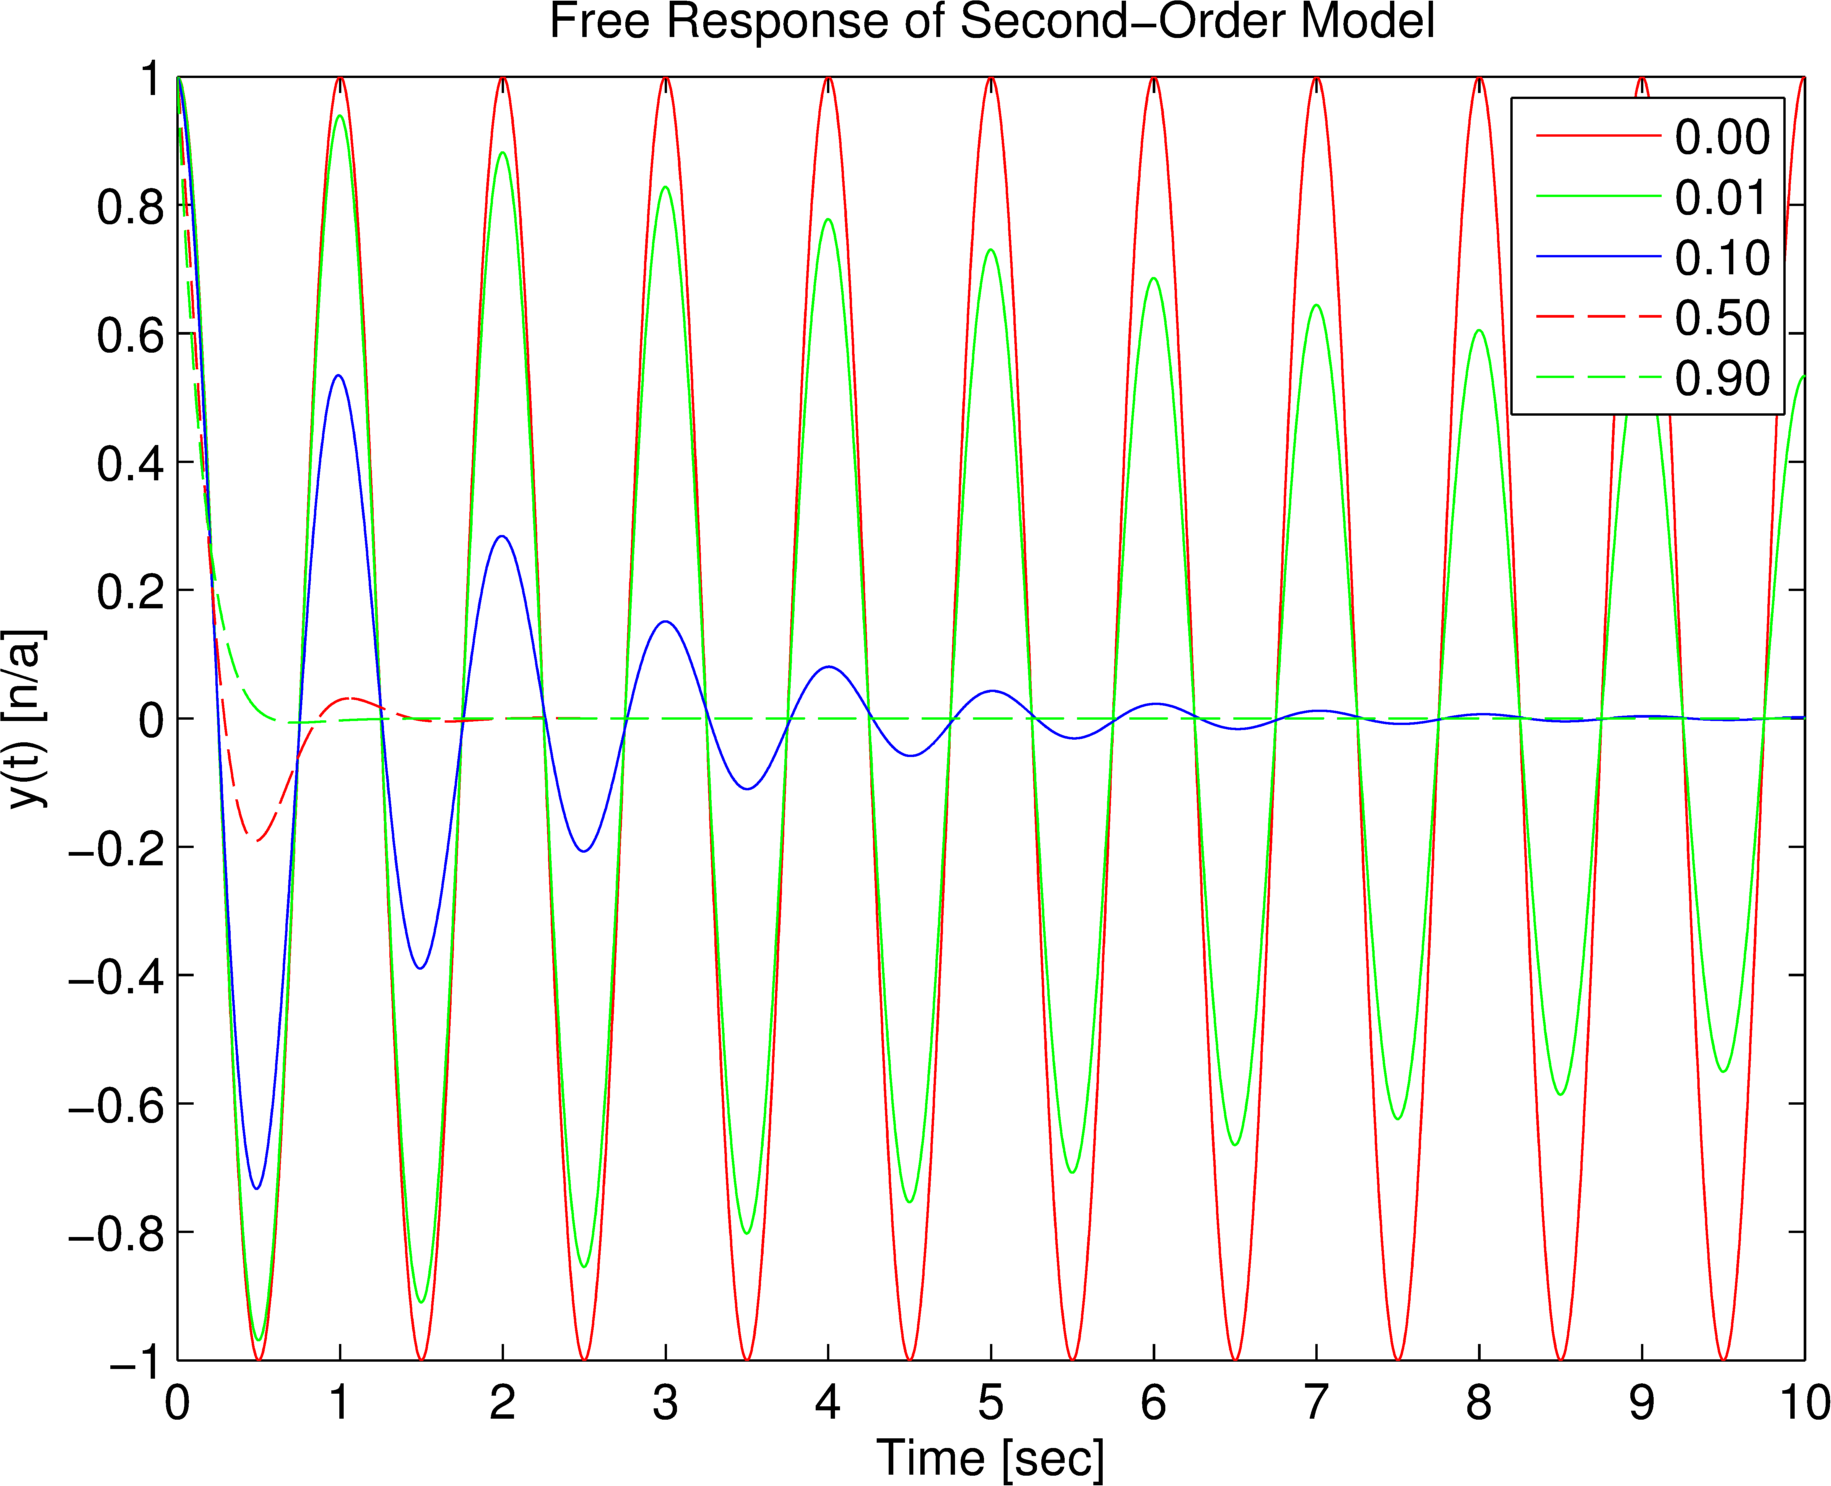
\includegraphics[width=\FigWidth\textwidth]{free_zetas.png}
\caption{}
\label{f:secondfreezetas}
\end{figure}

\end{soln}
\fi

\begin{ex}
Consider the model's free response to velocity-only initial conditions---$y(0)=0$ and $\dot{y}(0)=v_o$.
\begin{itemize}
\item Derive expressions for the constants $C$ and $\phi$ based on these initial conditions.
\item Substitute your expressions into the response (\ref{e:secondfree}) and write a simplified equation for the response.  (Hint: $\cos\left(u-\frac{\pi}{2}\right) = \sin(u)$.)
\item Using MATLAB, create a figure the graphs the response ($y(t)$) to this initial condition.
\end{itemize}
\end{ex}


\begin{ex}
Given a damping ratio of $\zeta=0.01$ (1\% damping), write and expression for the damped natural frequency as a function of the undamped natural frequency.  \\
Repeat the exercise for a 10\% damping.
\end{ex}

